\chapter{Предмет изучения химии}

\section{Что изучает химия}

\hspace*{\parindent}Для понимания роли химии в семействе естественных наук нам следует начать с ответа на вопрос~--- а что именно изучает химия, в чём её отличие от других наук, особенно физики?

\subsection*{Вещества}

Окружающий нас мир состоит из материи. Материю можно разделить на следующие виды:

\begin{itemize}
    \item \textbf{Вещество}\label{term:substance_matter}\index{вещество}~--- форма материи, обладающая массой. Вещество состоит из частиц, взаимодействующих между собой и организованных по определённым законам.
    \item \textbf{Поле}\label{term:field}\index{поле}~--- форма материи, посредством которой осуществляются взаимодействия между частицами вещества.
    \item \textbf{Прочие формы материи}~--- это формы невыясненной природы (тёмная материя и энергия), экзотические и гипотетические формы~--- (виртуальная, зеркальная, струноподобные объекты и пр.).
\end{itemize}

Физических полей в классическом понимании существует всего несколько типов, а вот формы организации вещества могут быть очень разнообразны. В Солнечной системе преобладает \textbf{барионная форма вещества}\label{term:baryonic_matter}\index{барионное вещество}. Так называют материю, состоящую из барионов (протонов, нейтронов) и электронов. Эти фун\-да\-мен\-таль\-ные, в свою очередь, организуются в более сложные образования~--- атомы, те~--- в ещё более сложные~--- молекулы, решётки и пр., а они, в свою очередь, в ещё более сложные формы и так далее. Наконец, если рассматривать вещество в ещё более укрупнённом виде, когда оно начинает представлять собой сплошную среду с точки зрения свойств, то происходит переход к макрообъектам, которые человек уже может видеть невооружённым взглядом.

\begin{figure}[htbp]
    \centering
    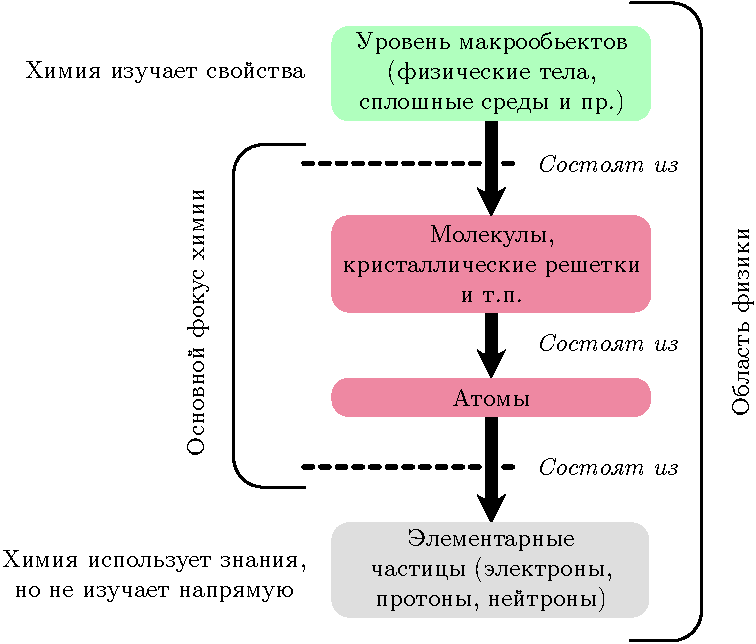
\includegraphics[width=9cm]{figs/chemistry_studies/levels_of_substance_structure.pdf}
    \caption{Уровни организации вещества, изучаемые химией.}
    \label{fig:levels_of_substance_structure}
\end{figure}

Человек, как существо, относящееся к макромиру и не способное воспринимать окружающие предметы на уровне элементарных частиц традиционно называет веществом просто \emph{то, из чего состоят объекты окружающего мира}, подразумевая под этим форму организации вещества как материи начиная от атомного и выше.\label{term:substance_human}

То есть, говоря о веществе, человек подразумевает, например, что гвозди изготовлены из железа, бутылка может быть изготовлена из стекла или пластмассы, а сложные предметы, например телевизор, изготовлены из большого количества разных веществ.

Химия как наука рассматривает вещество именно с такой точки зрения, не затрагивая субатомный уровень\footnote{\textbf{Субатомный уровень}\label{term:subatomic_level}\index{субатомный уровень}~--- рассмотрение вещества на уровне частиц размером меньше атома.} организации веществ, хотя очень активно использует знания об этом уровне в своих целях (рис.~\ref{fig:levels_of_substance_structure}).

Вещества могут изменяться~--- превращаться друг в друга. Например, железный гвоздь, помещённый в стакан с водой, начинает ржаветь. При этом одно вещество~--- железо, соединяется с кислородом и водой и превращается в другое вещество~--- ржавчину. Превращения одних веществ в другие называются \textbf{химическими реакциями}\label{term:chemical_reaction}\index{химическая реакция}.

Химические реакции, наряду с физическими процессами, постоянно происходят вокруг нас. Весь наш мир представляет собой непрекращающуюся череду таких изменений, включая функционирование нас как живых организмов. Даже наши мысли~--- это совокупность химических и физических процессов, происходящих в головном мозге.

\textbf{Химия}\label{term:chemistry}\index{химия}~--- это наука, которая изучает вещества и законы, по которым вещества превращаются друг в друга (т.~е. их \textbf{химические свойства}\label{term:chemical_properties}\index{химические свойства}).

Физика тоже исследует вещества на том же уровне организации материи, на котором их рассматривает и химия, однако не рассматривает превращения веществ друг в друга.

Если вещество рассматривается как макрообъект без детализации его структуры на уровне атомов, молекул и пр., то оно снова оказывается в области изучения физики и прекращает рассматриваться с точки зрения химии.

\subsection*{Различия между физикой и химией}

Таким образом, давайте сформулируем ключевые отличия между физикой и химией.

\textit{Предмет изучения}:

\begin{itemize}
    \item Физика исследует общие свойства и законы движения материи во всём многообразии форм: от элементарных частиц до космических систем. Фокус при этом~--- на взаимодействиях, силах, энергии, пространстве и времени.
    \item Химия изучает конкретные вещества, их состав, строение, свойства и превращения одних веществ в другие (химические реакции).
\end{itemize}

\textit{Масштаб и уровень описания}:

\begin{itemize}
    \item Физика работает на всех уровнях организации вещества~--- от субатомного (квантовая механика) до макроскопического (механика сплошных сред, астрофизика). Часто она абстрагируется от конкретного состава, фокусируясь на универсальных законах.
    \item Химия концентрируется на уровне атомов, молекул и ещё более сложных структурах. Её интересуют детали: как атомы соединяются, какие связи образуются, как меняется электронная оболочка.
\end{itemize}

\textit{Тип превращений}:

\begin{itemize}
    \item Физические процессы меняют состояние или форму вещества, но не его химический состав (например, плавление льда, испарение воды, деформация металла).
    \item Химические реакции приводят к образованию новых веществ с иным составом и свойствами (например, горение, окисление, синтез полимеров).
\end{itemize}

\textit{Цели исследования}:

\begin{itemize}
    \item Физика стремится выявить универсальные законы природы, объясняющие поведение материи на всех уровнях.
    \item Химия нацелена на понимание и управление химическими реакциями, создание новых материалов, лекарств, источников энергии.
\end{itemize}

Человек использует знания химии для получения новых веществ и защиты существующих от неблагоприятных воздействий. Многие вещества, например, большинство используемых человеком полимеров или биологически активных веществ не существуют в природе и получены искусственно. Получение веществ при помощи химических реакций называется \textbf{химическим синтезом}\label{term:chemical_synthesis}\index{химический синтез}.

Теперь вы легко справитесь с первой задачей (химикам приходится их решать постоянно в работе и в жизни), вот она:

\begin{problem}{}{chemistry_studies1}
    При описании тех или иных предметов часто употребляют слова, описывающие физические или химические характеристики вещества. Для следующих описаний предметов укажите, какие слова характеризуют физические, а какие химические свойства.
    \begin{enumerate}[label=\alph*)]
        \item старый ржавый нож;
        \item позеленевшая статуэтка;
        \item чистый прозрачный хрустальный графин;
        \item коричневый глиняный горшок.
    \end{enumerate}

    \begin{sol}{\ref{prob:chemistry_studies1}}
        О химических свойствах говорят слова, указывающие на способность вещества к реакциям. Поэтому химические свойства характеризуют следующие определения: ржавый (коррозия), позеленевшая (коррозия). Остальные слова характеризуют физические свойства (форму, цвет, прозрачность). Слова <<хрустальный>> и <<глиняный>> характеризуют \emph{состав материала}, а не химические свойства.
    \end{sol}
\end{problem}

Чтобы проверить себя, вы сможете найти все ответы в разделе~\nameref{sec:solutions}. Но постарайтесь сначала как следует подумать самостоятельно.

\subsection*{Физические и химические явления}

Теперь вы можете понять разницу между \textbf{физическими}\label{term:physical_phenomenon}\index{физические явления} и \textbf{химическими явлениями}\label{term:chemical_phenomenon}\index{химические явления}. В первом случае \emph{не происходит превращения одних веществ в другие}. Например: кипение, изгиб твёрдого тела, распространение звука, света и т.~п.

В случае химических явлений \emph{одни вещества превращаются в другие}, то есть они сопровождаются химической реакцией. В качестве примеров распространённых химических реакций можно привести горение, разрушение (коррозию) металлов, покрытие зелёным налётом медных изделий.

Химические и физические явления часто сопутствуют друг другу. Например, взрыв динамита -- явление химическое, однако он сопровождается физическими явлениями: шумом, светом, ударной волной взрыва и т.~п.

Более того, по наличию физических явлений часто судят о том, что происходит химическая реакция, например, по разогреванию смеси веществ после того, как их смешали.

Давайте решим следующую задачу.

\begin{problem}{}{chemistry_studies2}
    Как было сказано выше, химические реакции часто сопровождаются физическими явлениями, т.~е. \emph{характерными признаками}\label{term:signs_of_a_chemical_reaction}\index{признаки реакции}. Примеры таких признаков приведены в таблице ниже.
    
    \vspace{5pt}
    \begin{small}
    \begin{tabularx}{\textwidth}{|Y|Y|Y|Y|Y|}
        \hline
        \rowcolor{green!5}
        \multicolumn{5}{|c|}{Признаки химической реакции} \\
        \hline
        Изменение цвета исходного вещества &
        Изменение вкуса исходного вещества &
        Выпадение осадка &
        Выделение газа &
        Появление запаха \\
        \hline
    \end{tabularx}
    \end{small}
    \vspace{5pt}

    Для каждого признака приведите пример химического превращения (с которым можно встретиться в быту), при котором этот признак проявляется.

    \medskip

    Помните, что при химических реакциях всегда происходит превращение одних веществ в другие.

    \begin{sol}{\ref{prob:chemistry_studies2}}
        \noindent Для каждого признака можно указать примеры его проявления, например:
        \begin{itemize}
            \item \textit{Изменение цвета исходного вещества}: обугливание древесины при горении.
            \item \textit{Изменение вкуса исходного вещества}: скисание молока.
            \item \textit{Выпадение осадка}: кипячение жёсткой воды (образование накипи).
            \item \textit{Выделение газа}: выбросы автомобиля при сжигании топлива.
            \item \textit{Появление запаха}: порча пищевых продуктов.
        \end{itemize}
    \end{sol}
\end{problem}

Добавим к уже указанным в задаче ещё один важный признак химической реакции~--- выделение или поглощение теплоты. С выделением теплоты вы сталкиваетесь постоянно (например, при горении различных материалов). А вот охлаждение встречается реже, но изредка всё же происходит. Если растворить аммиачную селитру (продаётся как удобрение) в стакане с водой, то стакан настолько охладится, что даже примёрзнет к столу.

Также помните о том, что признаки~--- это не доказательства наличия химической реакции. Если мы смешаем две краски, то смесь изменит свой цвет, однако никакой химической реакции не произойдёт. Более того: реакции могут происходить вообще без всяких признаков.

\begin{problem}{}{chemistry_studies3}
    Некто \textit{профессор Недоумелкин} посетил ваши занятия и заявил, что он как никто другой разбирается в химии. <<Сейчас я продемонстрирую вам свои знания!>>,~--- воскликнул он.

    \medskip

    Профессор утверждает, что <<\emph{если вещество изменило цвет, это всегда химическая реакция!}>>. Приведите ещё один пример (кроме смешивания красок), чтобы опровергнуть его.

    \begin{sol}{\ref{prob:chemistry_studies3}}
        Нагревание металла до покраснения (изменение цвета из‑за температуры, без химической реакции).
    \end{sol}
\end{problem}

Теперь обдумайте понятия, указанные ниже в потоке терминов, и попытайтесь сформулировать, что означает каждое понятие. Если у вас возникают затруднения, то вы можете перейти по ссылкам в то место, где объясняется смысл термина. Прежде чем идти дальше, убедитесь, что вы хорошо понимаете то, что уже изучили.

\begin{termlist}
    \hyperref[term:substance_matter]{Вещество как вид материи}, 
    \hyperref[term:substance_human]{вещество в понимании человека}, 
    \hyperref[term:field]{поле}, 
    \hyperref[term:baryonic_matter]{барионная форма вещества}, 
    \hyperref[term:subatomic_level]{субатомный уровень}, 
    \hyperref[term:chemical_reaction]{химическая реакция}, 
    \hyperref[term:chemistry]{химия}, 
    \hyperref[term:chemical_properties]{химические свойства}, 
    \hyperref[term:chemical_synthesis]{химический синтез}, 
    \hyperref[term:physical_phenomenon]{физическое явление}, 
    \hyperref[term:chemical_phenomenon]{химическое явление}, 
    \hyperref[term:signs_of_a_chemical_reaction]{признаки химической реакции}.
\end{termlist}

Далее мы начнём изучать из чего состоят вещества, но, прежде давайте решим ещё несколько задач. Кстати, задачи посложнее мы будем обозначать звёздочкой $\bigstar$. Впрочем, их сложность~--- это наше субъективное мнение, вам они могут показаться довольно лёгкими. Так или иначе, если сумеете их решить, то это повод для гордости.

\begin{problem}{}{chemistry_studies4}
    Среди перечисленных процессов выберите химические явления:
    \begin{enumerate}[label=\alph*)]
        \item плавление льда;
        \item ржавление железа;
        \item скисание молока;
        \item выделение газа из газированных напитков;
        \item горение древесины;
        \item плавление железа.
    \end{enumerate}

    \begin{sol}{\ref{prob:chemistry_studies4}}
        Правильные ответы: b, c, e.
    \end{sol}
\end{problem}

\begin{problem}{}{chemistry_studies5}
    Какие из предложенных процессов являются физическими явлениями:
    \begin{enumerate}[label=\alph*)]
        \item образование зелёного налёта на медных предметах;
        \item покраснение раскалённого куска железа;
        \item радуга;
        \item растворение соли в воде;
        \item таяние снега;
        \item разложение воды электрическим током.
    \end{enumerate}

    \begin{sol}{\ref{prob:chemistry_studies5}}
        Правильные ответы: b, c, d, e. Растворение соли в воде является физическим явлением, так как не образуется новое вещество и процесс обратим (выпаривание возвращает соль в исходное состояние).
    \end{sol}
\end{problem}

\begin{problem}{}{chemistry_studies6}
    Приведите примеры химических реакций, которые начинаются из-за физического воздействия.

    \begin{sol}{\ref{prob:chemistry_studies6}}
        Главная идея для поиска~--- физическое воздействие должно передать веществам энергию для того, чтобы они начали реагировать. Примеры: инициирование горения поджиганием (по сути~--- нагревание), протекание фотосинтеза под действием света, взрыв пороха, выцветание краски на солнце и т.~п. 
    \end{sol}
\end{problem}

\begin{problem}{}{chemistry_studies7}
    Подумайте, какие из окружающих вас веществ человек добывает из природы, а какие синтезирует искусственно.

    \begin{sol}{\ref{prob:chemistry_studies7}}
        Добывает из природы: например, древесина, сахар, крахмал, шерсть, морская соль. Синтезирует искусственно: пластмассы, краски, бензин, лекарственные препараты и пр.
    \end{sol}
\end{problem}

\begin{problem}{}{chemistry_studies8}
    Опишите три химических процесса, которые происходят на кухне во время приготовления пищи. Укажите признаки реакций (выделение газа, изменение цвета и т.~п.).

    \begin{sol}{\ref{prob:chemistry_studies8}}
        \begin{itemize}
            \item Подгорание хлеба (изменение цвета, появление запаха).
            \item Гашение соды уксусом (выделение газа).
            \item Скисание молока (изменение вкуса, образование осадка).
        \end{itemize}
    \end{sol}
\end{problem}

\begin{problem}{}{chemistry_studies9}
    $\bigstar$ Бывает так, что один и тот же процесс изучают сразу несколько наук. Объясните, почему фотосинтез изучают и в химии, и в биологии. Чем отличаются их подходы?

    \begin{sol}{\ref{prob:chemistry_studies9}}
        Химия: изучает химические реакции (превращение углекислого газа и воды в глюкозу, как участвует хлорофилл в химической реакции). Биология рассматривает фотосинтез как часть процесса жизнедеятельности растений, а также его роль в экосистемах.
    \end{sol}
\end{problem}

\begin{problem}{}{chemistry_studies10}
    $\bigstar$ Приведите примеры веществ, которые встречаются в природе, но которые человек предпочитает синтезировать самостоятельно в силу каких-либо причин. Подумайте, какие это могут быть причины? Не стесняйтесь пользоваться информацией в интернете.

    \begin{sol}{\ref{prob:chemistry_studies10}}
        Например, каучук, который получают из млечного сока деревьев рода Гевея. Однако большую его часть сейчас синтезируют из нефти. Причины, почему синтезируют тот или иной продукт, а не добывают из природных источников, всегда экономические, технологические или практические:
        \begin{itemize}
            \item Природные ресурсы не могут предоставить нужного количества продукта (к примеру, нельзя засадить каучуконосными растениями полземли).
            \item Промышленный процесс позволяет лучше контролировать качество продукта.
            \item Можно получать продукт с заданными свойствами или с гораздо более высоким качеством, чем природный.
        \end{itemize}
    \end{sol}
\end{problem}

\begin{problem}{}{chemistry_studies11}
    $\bigstar$ Приведите примеры веществ, которые человек способен синтезировать самостоятельно, но предпочитает добывать их из природных источников. Почему так происходит?

    \begin{sol}{\ref{prob:chemistry_studies11}}
        Человек использует природные ресурсы, если их использование дешевле, чем синтез искусственных, синтез слишком сложен либо имеющиеся природные ресурсы более, чем достаточны для покрытия потребления. Пара примеров: углеводороды, поваренная соль, известняк (мел), натуральные масла и жиры.
    \end{sol}
\end{problem}

\begin{problem}{}{chemistry_studies12}
    $\bigstar$ После долгого и упорного обучения вы, наконец, в совершенстве овладели знаниями химии и теперь раздумываете, чем бы заняться. Предложите два новых вещества, которые вы попробуете синтезировать искусственно. Почему они будут важны для человечества?

    \begin{sol}{\ref{prob:chemistry_studies12}}
        Много вариантов, например, саморазлагающийся пластик из водорослей (чтобы снизить проблему загрязнения океанов мусором), искусственный гемоглобин для создания крови для переливания без использования доноров.
    \end{sol}
\end{problem}

\clearpage

\section{Химические элементы и формулы}

\begin{wrapfigure}{l}{0.17\textwidth}
    \centering
    
\includegraphics[width=1.8cm]{figs/what_is_a_chemical_element/frog.pdf}
\end{wrapfigure}

\hspace*{\parindent}На самом деле, для того, чтобы осуществить задуманное (в том числе и в обучении) разумно использовать известный подход из тайм-менеджмента (навыков разумного использования своего времени)~--- <<\emph{как съесть лягушку?}>> и <<\emph{как съесть слона?}>>.

<<Лягушка>>~--- это неприятная, но обычно небольшая задача, которую хочется отложить. Как её решить? Съесть и всё. То есть сделать сразу, недолго думая.

\begin{wrapfigure}{r}{0.3\textwidth}
    \centering
    
\includegraphics[width=3.5cm]{figs/what_is_a_chemical_element/elephant.pdf}
\end{wrapfigure}

Изучение химии~--- это <<Слон>>: масштабная задача, которая пугает своими размерами. Слона нужно есть по частям, то есть разделить изучение на маленькие части (бифштексы) и действовать регулярно и постепенно. В этом случае успех неизбежен.

Итак, как мы выяснили, область изучения химии ограничена <<снизу>> атомным уровнем. То есть химики не рассматривают то, как устроены составляющие атом частицы, хотя используют физические знания об устройстве атома и взаимодействии субатомных частиц.

<<Сверху>> химия ограничена организацией атомов между собой на микроуровне, то есть рассматривает объединения атомов, их связи, структуру образующихся объединений и превращение их друг в друга до тех пор, пока вещество не начинает рассматриваться как макрообъект.

\textbf{Атом}\label{term:atom}\index{атом}~--- это наименьшая химически неделимая частица вещества. <<Химически неделимая>> означает, что никакими химическими реакциями невозможно разрушить атом, только изменить его связи с другими атомами. Атомы бывают разных видов, каждый со своими уникальными физическими и химическими свойствами.

Атомы определённого вида называют \textbf{химическими элементами}\label{term:chemical_element}\index{химический элемент}, например, хлор, аргон, кислород.

При помощи химических реакций атом невозможно превратить в другой химический элемент, но это можно сделать посредством \emph{ядерных реакций}.

Атомы могут взаимодействовать друг с другом, образуя \textbf{химическую связь}\label{term:chemical_bond}\index{химическая связь}. Образование химической связи выгодно с точки зрения энергии, то есть атомы, связанные химической связью, имеют меньшую энергию, чем отдельные изолированные атомы.

Вещества, как правило, представляют собой повторяющиеся устойчивые совокупности атомов, связанные химическими связями. Графически это обычно представляют в виде атомов, соединённых линиями различного вида, как, например, на рис.~\ref{fig:chemical_bond}.

\begin{figure}[htbp]
    \centering
    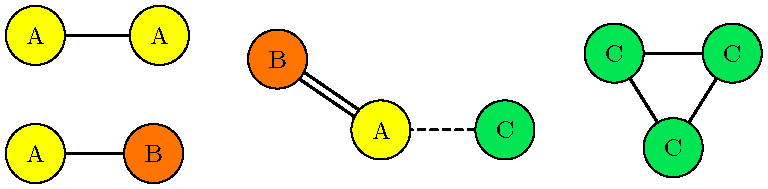
\includegraphics[width=7.5cm]{figs/what_is_a_chemical_element/chemical_bond.pdf}
    \caption{Связи между атомами можно изображать в виде линий различного типа.}
    \label{fig:chemical_bond}
\end{figure}

Вещества делят на простые и сложные. \textbf{Простые вещества}\label{term:chemical_element_substance}\index{простое вещество} состоят из атомов одного химического элемента. Называют простые вещества, за некоторым исключением, так же, как и сами химические элементы: железо, бром, сера.

\textbf{Сложные вещества}\label{term:chemical_compound}\index{сложное вещество} (или \textbf{химические соединения}) состоят из атомов как минимум двух различных химических элементов. Например, хлорид натрия состоит из атомов натрия и хлора.

\subsection*{Химическая азбука}

В химии, как и в любой другой науке, для того, чтобы каждый специалист из любой точки мира мог понимать любого другого специалиста, используется свой стандартный язык и обозначения. Особенно важную его часть занимает стандартизация того, как правильно обозначать и называть химические элементы и их соединения, особенно если учесть тот факт, что число последних исчисляется десятками миллионов.

Занимается такой стандартизацией \href{https://iupac.org}{ИЮПАК} (IUPAC)~---  Международный союз теоретической и прикладной химии (\textit{International Union of Pure and Applied Chemistry}),~--- это организация, которая разрабатывает и утверждает правила <<химического языка>>.

Какие же договорённости приняты в этой области касаемо химических элементов? Чтобы отличать химические элементы друг от друга, используют две их главные характеристики~--- название и обозначение на письме.

Обозначают химические элементы одной или двумя буквами латинского алфавита, например, \ce{Na}, \ce{S}, \ce{Fe}, \ce{O} и др. ИЮПАК придерживается правила, согласно которому все новые открытые химические элементы будут получать только двухбуквенные обозначения.

В русском языке исторически сложилось так, что названия химических элементов различаются в зависимости от того, в какой ситуации мы их называем. Есть два типа названий (табл.~\ref{tab:elements_name}), каждое из которых служит для определённых целей:

\begin{itemize}
    \item русское название;
    \item латинское название.
\end{itemize}

Особняком стоит вопрос наименования химических элементов \emph{при чтении формул} соединений для элементов, которые обозначаются одной буквой (углерод \ce{C}, азот \ce{N} и др.). Их названия произносят так, как они произносятся по-русски. Примеры таких элементов также имеются в (табл.~\ref{tab:elements_name}).

\begin{table}
    \small
    \caption{Примеры названий химических элементов.}
    \label{tab:elements_name}
    \begin{tabularx}{\textwidth}{
        >{\hsize=0.8\hsize}Y
        >{\hsize=0.8\hsize}Y
        >{\hsize=0.9\hsize}Y
        >{\hsize=1.5\hsize}Y
        }
        \hline
        \rowcolor{green!5}
        Обозначение\newline химического\newline элемента &
        Русское\newline название &
        Латинское\newline название & 
        Чтение буквенного обозначения на русском языке в формулах \\
        \hline
        \ce{H} &
        Водород &
        \textit{Hydrogenium} &
        <<аш>> \\
        \ce{Be} &
        Бериллий &
        \textit{Beryllium} &
        - \\
        \ce{C} &
        Углерод &
        \textit{Carboneum} &
        <<це>> \\
        \ce{O} & 
        Кислород &
        \textit{Oxygenium} &
        <<о>> \\
        \ce{F} &
        Фтор &
        \textit{Fluorum} &
        <<эф>> \\
        \hline
    \end{tabularx}
\end{table}

Русское и латинское названия для каждого из открытых на данный момент химических элементов приведены в приложении~\ref{appendix:Russian_and_Latin_names_of_chemical_elements}. Также русское название для всех элементов обычно присутствует в периодической таблице химических элементов, речь о которой пойдёт чуть позже.

Для того, чтобы показать, какие химические элементы и в каком количестве содержатся в веществе (а также дополнительную информацию), используют \textbf{формулы химических соединений}. Химические элементы в формулах записывают при помощи их буквенных обозначений. Существует несколько типов формул, предназначенных для определённых целей (рис.~\ref{fig:types_of_formulas}).

\begin{figure}[htbp]
    \centering
    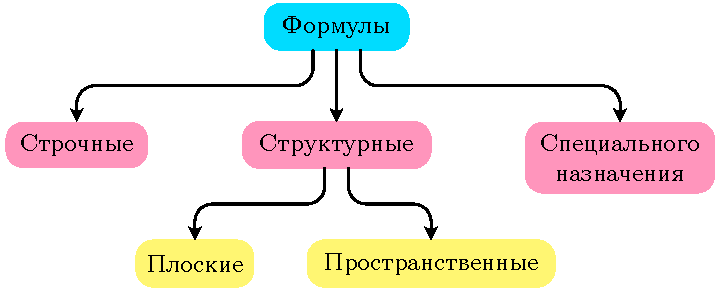
\includegraphics[width=9cm]{figs/what_is_a_chemical_element/types_of_formulas.pdf}
    \caption{Типы формул химических соединений.}
    \label{fig:types_of_formulas}
\end{figure}

\subsection*{Строчные формулы}

\textbf{Строчные формулы}\label{term:formula_in_row}\index{строчная формула} являются самыми простыми и показывают, какие атомы и в каком соотношении имеются в химическом соединении. При этом в строчку записывают буквенные обозначения химических элементов и нижним правым индексом~--- число атомов этого элемента. Например:

\begin{itemize}
    \item \ce{H2O}~--- вода, молекула которой состоит из двух атомов водорода и одного атома кислорода;
    \item \ce{H2SO4}~--- серная кислота. В её молекуле два атома водорода, один~--- серы и четыре~--- кислорода.
\end{itemize}

Если какая-либо группа атомов повторяется в соединении многократно в виде \emph{устойчивой группы}, связанной внутри себя химическими связями, то ее выделяют в формуле круглыми скобками и правым нижним индексом записывают число таких групп, например:

\begin{itemize}
    \item \ce{Fe2(SO4)3}~--- сульфат железа, имеет три сульфатных группы \ce{SO4};
    \item \ce{Ba(OH)2}~--- гидроксид бария, содержит две гидроксидные группы \ce{OH}.
\end{itemize}

Термин <<устойчивая группа>> означает, что атомы, записанные в скобках, действительно находятся рядом друг с другом в соединении и связаны между собой. Например, формулу гипохлорита кальция записывают именно как \ce{Ca(OCl)2}, а не как \ce{Cl2CaO2} и не как \ce{CaO2Cl2}, чтобы показать, что в соединении существуют устойчивые гипохлоритные группы \ce{OCl}, что хорошо видно, если записать структурную формулу этого соединения.

\subsection*{Структурные формулы}

\textbf{Плоская структурная формула}\label{term:planar_structural_formula}\index{плоская структурная формула} показывает в какой последовательности атомы соединены между собой связями в химическом соединении, как, например, в молекулах воды и серной кислоты (рис.~\ref{fig:molecules_examples}). Также из структурной формулы можно понять, сколько связей имеется между теми или иными атомами в соединении.

\begin{figure}[htbp]
    \centering
    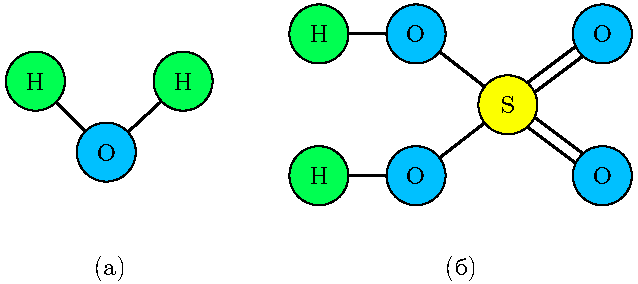
\includegraphics[width=6.2cm]{figs/what_is_a_chemical_element/molecules_examples.pdf}
    \caption{Плоские структурные формулы молекул воды (а) и серной кислоты (б).}
    \label{fig:molecules_examples}
\end{figure}

Из структурной формулы рассматривавшегося выше гипохлорита кальция мы можем понять, что гипохлоритная группа действительно является <<устойчивой группой>>, так как атомы, входящие в состав этой группы, связаны между собой (рис.~\ref{fig:calcium_hypochlorite}).

\begin{figure}[htbp]
    \centering
    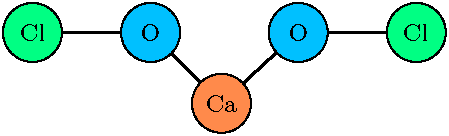
\includegraphics[width=4.4cm]{figs/what_is_a_chemical_element/calcium_hypochlorite.pdf}
    \caption{Структурная формула гипохлорита кальция.}
    \label{fig:calcium_hypochlorite}
\end{figure}

Из плоских структурных формул можно увидеть, в какой последовательности связаны атомы в веществе, но невозможно понять, как эти атомы располагаются в пространстве, например, какую форму имеет молекула соединения. Для информации о взаимном расположении атомов используют \textbf{пространственные структурные формулы}\label{term:spatial_structural_formula}\index{пространственная структурная формула}. Они представляют собой трёхмерные изображения, на которых атомы обычно изображают в виде шариков либо их буквенными наименованиями, а связи~--- в виде линий различного вида.

\begin{figure}[htbp]
    \centering
    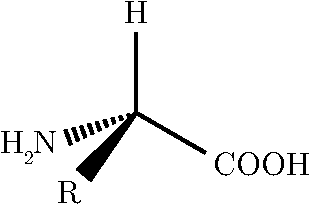
\includegraphics[width=3.2cm]{figs/what_is_a_chemical_element/amino_acid.pdf}
    \caption{Пространственная структурная формула аминокислоты.}
    \label{fig:amino_acid}
\end{figure}

Например, на рис.~\ref{fig:amino_acid} изображена общая пространственная формула молекулы аминокислоты (эти соединения входят в состав белков в живых организмах). Связи, находящиеся в плоскости рисунка, обозначены обычными линиями. Сплошные треугольные линии связи означают, что они выходят из плоскости рисунка по направлению к нам, а пунктирные треугольные~--- от нас.

\subsection*{Формулы специального назначения}

Особняком стоят специальные формулы, которые зачастую даже не предназначены для чтения их человеком. Обычно задача таких формул~--- представить формулу вещества в виде, удобном для компьютерной обработки. Также их часто называют <<формулы для машин>>. Часто, хотя не всегда, такие формулы разработаны с таким расчётом, чтобы можно было однозначно идентифицировать вещество (не было двух разных веществ с одинаковой формулой).

Например, к таким формулам можно отнести формулы \textbf{SMILES} (\textit{Simplified Molecular Input Line Entry System}), которые представляют собой строку из символов. Кодировка происходит следующим образом:

\begin{itemize}
    \item атомы обозначают их символами (\ce{C}, \ce{F}, \ce{H} и др.);
    \item связи между ними обозначают специальными символами: одинарные не обозначают, двойные обозначают как =, тройные~--- как \#;
    \item ответвления обозначают скобками;
    \item циклические структуры обозначают, ставя цифры после атомов, между которыми есть связь;
    \item после определения <<скелета>> молекулы, оставшиеся связи, которые должны присутствовать, заполняют атомами водорода.
\end{itemize}

Например:

\begin{itemize}
    \item \fbox{\textcolor{blue}{O}}~--- вода;
    \item \fbox{\textcolor{blue}{C\#C}}~--- ацетилен;
    \item \fbox{\textcolor{blue}{CC(=O)Oc1ccccc1C(=O)O}}~--- ацетилсалициловая кислота (Аспирин).
\end{itemize}

Такие формулы обычно используются в базах данных химических соединений, различных каталогах, в машинном обучении, при автоматизированном планировании синтеза соединений и т.~п. Систем формул специального назначения существует довольно много\footnote{Например, очень известна система \textbf{InChI} (\textit{IUPAC International Chemical Identifier}), более строгая и стандартизированная, чем \textbf{SMILES}.}.

\subsection*{Русские названия элементов}

Теперь давайте разберёмся с применением каждого варианта наименования элементов. Начнём с русского названия. Если мы подразумеваем элемент как разновидность атомов, то просто произносим его русское название. Например: <<\emph{в этом минерале высокое содержание свинца}>> или <<\emph{иод является важным микроэлементом}>>. Также русское название используется при чтении строчных формул для части элементов, об этом чуть позже.

Не путайте понятия \emph{химический элемент} и \emph{простое вещество}, в речи они произносятся одинаково~--- русским названием. Химический элемент~--- это разновидность атомов, а простое вещество~--- это вещество, состоящее из атомов одного химического элемента.

О чём идёт речь можно понять только из контекста. Сравните, например, <<\emph{натрий проявляет высокую металличность}>> (говорим о химическом элементе) и <<\emph{произошла утечка жидкого натрия из трубопровода на АЭС}>> (говорим о простом веществе).

\subsection*{Латинские названия элементов}

С латинскими названиями ситуация более интересная. У них два применения:

\begin{itemize}
    \item для формирования названия соединения по номенклатуре ИЮПАК;
    \item при чтении строчных формул на русском языке для некоторых элементов.
\end{itemize}

\textbf{Номенклатурой химических соединений}\label{term:chemical_nomenclature}\index{номенклатура} называют правила, по которым строятся их названия. Те правила, которые приняты ИЮПАК, называют \emph{научной номенклатурой}: это хорошо продуманная система, логичная и однозначная, не привязанная к историческим традициям.

Например, <<дигидрофосфат калия>>, <<сернистая кислота>>~--- это научные названия соединений. По ним нельзя осуществить <<обратное преобразование>> в строчную формулу, если вы не знаете правил номенклатуры. Правила номенклатуры ИЮПАК мы будем изучать постепенно по мере знакомства с различными классами соединений.

В правилах ИЮПАК используются латинские названия химических элементов. Например, в названии вещества <<сульфид железа>> \ce{FeS} используется корень из латинского названия серы~--- \textit{\textcolor{blue}{Sulf}ur}. 

Также латинские названия используются в русском языке для чтения строчных формул, но только для некоторых элементов, которые известны давно и прочно укоренились в своих традиционных латинских названиях. Эти элементы приведены в табл.~\ref{tab:latin_name_for_elements}, запомните их.

\begin{table}
    \small
    \caption{Для этих элементов используйте латинские названия при чтении формул. *Платина может читаться как в латинском, так и в русском вариантах.}
    \label{tab:latin_name_for_elements}
    \begin{tabularx}{\textwidth}{YY}
        \hline
        \rowcolor{green!5}
        Элемент & Латинское название \\
        \hline
        \ce{Fe} (Железо) & Ferrum (чит. <<феррум>>) \\
        \ce{Cu} (Медь) & Cuprum (чит. <<купрум>>) \\
        \ce{As} (Мышьяк) & Arsenicum (чит. <<арсеникум>>) \\
        \ce{Ag} (Серебро) & Argentum (чит. <<аргентум>>) \\
        \ce{Sn} (Олово) & Stannum (чит. <<станнум>>) \\
        \ce{Sb} (Сурьма) & Stibium (чит. <<стибиум>>) \\
        \ce{Pt} (Платина)* & Platinum (чит. <<платинум>>) \\
        \ce{Au} (Золото) & Aurum (чит. <<аурум>>) \\
        \ce{Hg} (Ртуть) & Hydrargyrum (чит. <<гидраргирум>>) \\
        \ce{Pb} (Свинец) & Plumbum (чит. <<плюмбум>>) \\
        \hline
    \end{tabularx}
\end{table}

\subsection*{Чтение строчных формул}\label{sec:reading_lowercase_formulas}

Номенклатура ИЮПАК не предоставляет правил <<для зачитывания>> формул, только для научного названия веществ, однако часто химики при общении друг с другом просто зачитывают формулу по элементам с указанием количества атомов, например формулу воды \ce{H2O} зачитывают как <<аш два о>>. Вероятно, раньше использовали латинские названия для всех элементов, но исторически из-за длинного и неудобного произношения в русском языке названия почти всех двухбуквенных химических элементов стали произносить как русские названия, а однобуквенных~--- так, как произносятся буквы, которыми они записаны. Например, никто не читает название оксида натрия \ce{Na2O} как <<натриум два оксигениум>>, а читают как <<натрий два о>>.

Тем не менее элементы, которые мы указали в табл.~\ref{tab:latin_name_for_elements}, продолжают читаться по-латински и в настоящее время. Например формулу оксида мышьяка \ce{As2O3} читают как <<арсеникум два о три>>.

Некоторые химические элементы обозначаются одной буквой, например, \ce{B}~--- бор, \ce{S}~--- сера и т.~д. Как уже было указано выше, при зачитывании формул соединений, содержащих эти элементы, просто произносят буквенные обозначения.

Когда вы встречаете строчную формулу химического соединения, вы можете прочитать её двумя способами:

\begin{itemize}
    \item как название химического соединения по правилам номенклатуры;
    \item зачитать формулу через составляющие её химические элементы.
\end{itemize}

Первый способ предполагает, что вы владеете знаниями номенклатуры химических соединений. Второй способ~--- просто зачитать формулу так, как она записана. Для этого необходимо использовать правила применения названий элементов, указанные выше. Например:

\begin{itemize}
    \item \ce{H2O}~--- <<аш два о>>;
    \item \ce{CaCl2}~--- <<кальций хлор два>>;
    \item \ce{SO2}~--- <<эс о два>>.
\end{itemize}

Если в формуле есть устойчивые группы, то их количество зачитывают после чтения формулы самой группы, например:

\begin{itemize}
    \item \ce{Ca(OH)2}~--- <<кальций о аш дважды>>;
    \item \ce{Fe2(SO4)3}~--- <<феррум два эс о четыре трижды>>;
    \item \ce{Cu3(PO4)2}~--- <<купрум три пэ о четыре дважды>>.
\end{itemize}

\begin{problem}{}{what_is_a_chemical_element1}
    Попрактикуемся в чтении строчных формул. Прочтите те, что указаны ниже:
    \begin{enumerate}
        \item \ce{LiCl};
        \item \ce{HgBr2};
        \item \ce{AgNO3};
        \item \ce{Fe(OH)3}.
    \end{enumerate}

    \begin{sol}{\ref{prob:what_is_a_chemical_element1}}
        \begin{enumerate}
            \item <<литий хлор>>;
            \item <<гидраргирум бром два>>;
            \item <<аргентум эн о три>>;
            \item <<феррум о аш трижды>>.
        \end{enumerate}
    \end{sol}
\end{problem}

\subsection*{Периодическая таблица химических элементов~--- знакомство}

Давайте начнём знакомство с \hyperref[appendix:periodic_table]{периодической таблицей химических элементов} (также в русскоязычной литературе её называют таблицей Менделеева\footnote{Правда, в других странах её так не называют, поэтому лучше использовать название <<периодическая таблица химических элементов>>.}). Знакомиться с ней мы будем постепенно, по мере углубления знаний о химических элементах.

Рассмотрите эту таблицу. В ней каждая клетка содержит один из химических элементов и информацию о нём, которую туда поместили составители таблицы. Как минимум, в каждой клетке будет находиться название элемента и его буквенное обозначение. Столбцы таблицы называют \emph{группами}, а строки~--- \emph{периодами}. Каждый химический элемент имеет порядковый номер~--- так называемый \emph{атомный номер} (рис.~\ref{fig:element_example}).

Периоды традиционно обозначаются арабскими цифрами а группы~--- римскими. В группах имеются две подгруппы~--- главная и побочная, обозначаемые латинскими буквами. Главная подгруппа обозначается буквой <<a>>, а побочная~--- <<b>>. Например, углерод относится к группе IVa, а титан~--- к IVb.

Данная нумерация групп в периодической таблице на самом деле является устаревшей, но тем не менее по-прежнему используется в русскоязычной литературе (и частично на территории стран бывшего СССР). Международный стандарт ИЮПАК (с 1988 года) рекомендует нумерацию групп арабскими цифрами от 1 до 18. Именно эту версию вы будете встречать при работе с литературой на иностранном языке. Эти две версии периодической таблицы называют \emph{короткопериодной} и \emph{длиннопериодной}.

\begin{figure}[htbp]
    \centering
    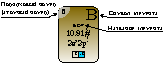
\includegraphics[width=8cm]{figs/what_is_a_chemical_element/element_example.pdf}
    \caption{Основные обозначения химического элемента в периодической таблице.}
    \label{fig:element_example}
\end{figure}

Русские названия и буквенные обозначения для каждого химического элемента химик должен знать наизусть. Для начала, выучите их для первых двадцати химических элементов.

Проверьте, можете ли вы дать определение всем терминам из потока терминов. Если нет, то повторите соответствующую часть раздела.

\begin{termlist}
    \hyperref[term:atom]{Атом}, 
    \hyperref[term:chemical_element]{химический элемент}, 
    \hyperref[term:chemical_bond]{химическая связь}, 
    \hyperref[term:chemical_element_substance]{простое вещество}, 
    \hyperref[term:chemical_compound]{сложное вещество}, 
    \hyperref[term:planar_structural_formula]{структурная формула},
    \hyperref[term:spatial_structural_formula]{пространственная структурная формула},
    \hyperref[term:formula_in_row]{строчная формула}, 
    \hyperref[term:chemical_nomenclature]{номенклатура}.
\end{termlist}

Изучите периодическую таблицу химических элементов и решите задачи ниже.

\begin{problem}{}{what_is_a_chemical_element2}
    Ответьте на следующие вопросы:
    \begin{enumerate}[label=\arabic*)]
        \item Сколько на данный момент открыто химических элементов?
        \item Сколько элементов содержится в группе 7b? А 3b?
        \item Какой период содержит меньше всего элементов? А какие больше всего?
        \item Каких химических элементов больше~--- металлов или неметаллов? При ответе постарайтесь вспомнить элементы, с которыми вы сталкивались в жизни.
        \item По названиям химических элементов постарайтесь догадаться, какие из них были названы в честь небесных тел?
    \end{enumerate}

    \begin{sol}{\ref{prob:what_is_a_chemical_element2}}
        \begin{enumerate}[label=\arabic*)]
            \item 118.
            \item 4 и 32. Обратите внимание, что некоторые периоды, содержащие большое количество элементов, сокращают: элементы группируют в одной клетке, а затем показывают в нижней части таблицы. Эти две группы элементов называют лантаноидами и актиноидами.
            \item 1 период, 6 и 7 периоды.
            \item Металлов.
            \item Гелий, селен, теллур, уран, нептуний, плутоний, церий и палладий.
        \end{enumerate}
    \end{sol}
\end{problem}

\begin{problem}{}{what_is_a_chemical_element3}
    Прочитайте строчные формулы с использованием \hyperref[sec:reading_lowercase_formulas]{правил чтения химических элементов}:
    \begin{enumerate}
        \item \ce{AlCl3};
        \item \ce{SnI2};
        \item \ce{SO2Cl2};
        \item \ce{Pb(CH3COO)2}.
    \end{enumerate}

    \begin{sol}{\ref{prob:what_is_a_chemical_element3}}
        \begin{enumerate}
        \item <<алюминий хлор три>>;
        \item <<станнум иод два>>;
        \item <<эс о два хлор два>>;
        \item <<плюмбум це аш три це о два дважды>>.
    \end{enumerate}
    \end{sol}
\end{problem}

\begin{problem}{}{what_is_a_chemical_element4}
    Составьте химические формулы по тому, как вам их зачитали.
    \begin{enumerate}
        \item <<аргентум эн о три>>;
        \item <<аш два эс о три>>;
        \item <<аш два о два>>;
        \item <<це о>>.
    \end{enumerate}

    \begin{sol}{\ref{prob:what_is_a_chemical_element4}}
        \begin{enumerate}
        \item \ce{AgNO3};
        \item \ce{H2SO3};
        \item \ce{H2O2};
        \item \ce{CO}.
    \end{enumerate}
    \end{sol}
\end{problem}

\begin{problem}{}{what_is_a_chemical_element5}
    $\bigstar$ В периодической таблице есть сразу четыре химических элемента, названных в честь маленького шведского городка Иттербю (\textit{Ytterby}). Попытайтесь по названиям догадаться, что это за элементы. Затем найдите информацию, чем же так прославился этот город?

    \begin{sol}{\ref{prob:what_is_a_chemical_element5}}
        Иттрий (\ce{Y})~--- открыт в 1794~году финским химиком Юханом Гадолином в минерале, найденном близ Иттербю.

        Тербий (\ce{Tb})~--- выделен в 1843~году шведским химиком Карлом-Густавом Мосандером из оксида иттрия.

        Эрбий (\ce{Er})~--- также открыт Мосандером в 1843~году в том же образце.

        Иттербий (\ce{Yb})~--- обнаружен в 1878~году швейцарским химиком Жаном де Мариньяком в оксиде эрбия.

        Почему именно Иттербю?

        В окрестностях этого населённого пункта (на острове Ресарё Стокгольмского архипелага) находится рудник, где в 1787~году офицер Карл Аксель Аррениус нашёл минерал гадолинит (первоначально названный <<иттербитом>>). Этот минерал оказался богатейшим источником редкоземельных элементов. В нём впоследствии были открыты не только четыре элемента, названные в честь Иттербю, но и другие (скандий, тулий, лютеций, гадолиний), хотя их названия связаны уже с иными объектами.
    \end{sol}
\end{problem}